\documentclass[1p]{elsarticle_modified}
%\bibliographystyle{elsarticle-num}

%\usepackage[colorlinks]{hyperref}
%\usepackage{abbrmath_seonhwa} %\Abb, \Ascr, \Acal ,\Abf, \Afrak
\usepackage{amsfonts}
\usepackage{amssymb}
\usepackage{amsmath}
\usepackage{amsthm}
\usepackage{scalefnt}
\usepackage{amsbsy}
\usepackage{kotex}
\usepackage{caption}
\usepackage{subfig}
\usepackage{color}
\usepackage{graphicx}
\usepackage{xcolor} %% white, black, red, green, blue, cyan, magenta, yellow
\usepackage{float}
\usepackage{setspace}
\usepackage{hyperref}

\usepackage{tikz}
\usetikzlibrary{arrows}

\usepackage{multirow}
\usepackage{array} % fixed length table
\usepackage{hhline}

%%%%%%%%%%%%%%%%%%%%%
\makeatletter
\renewcommand*\env@matrix[1][\arraystretch]{%
	\edef\arraystretch{#1}%
	\hskip -\arraycolsep
	\let\@ifnextchar\new@ifnextchar
	\array{*\c@MaxMatrixCols c}}
\makeatother %https://tex.stackexchange.com/questions/14071/how-can-i-increase-the-line-spacing-in-a-matrix
%%%%%%%%%%%%%%%

\usepackage[normalem]{ulem}

\newcommand{\msout}[1]{\ifmmode\text{\sout{\ensuremath{#1}}}\else\sout{#1}\fi}
%SOURCE: \msout is \stkout macro in https://tex.stackexchange.com/questions/20609/strikeout-in-math-mode

\newcommand{\cancel}[1]{
	\ifmmode
	{\color{red}\msout{#1}}
	\else
	{\color{red}\sout{#1}}
	\fi
}

\newcommand{\add}[1]{
	{\color{blue}\uwave{#1}}
}

\newcommand{\replace}[2]{
	\ifmmode
	{\color{red}\msout{#1}}{\color{blue}\uwave{#2}}
	\else
	{\color{red}\sout{#1}}{\color{blue}\uwave{#2}}
	\fi
}

\newcommand{\Sol}{\mathcal{S}} %segment
\newcommand{\D}{D} %diagram
\newcommand{\A}{\mathcal{A}} %arc


%%%%%%%%%%%%%%%%%%%%%%%%%%%%%5 test

\def\sl{\operatorname{\textup{SL}}(2,\Cbb)}
\def\psl{\operatorname{\textup{PSL}}(2,\Cbb)}
\def\quan{\mkern 1mu \triangleright \mkern 1mu}

\theoremstyle{definition}
\newtheorem{thm}{Theorem}[section]
\newtheorem{prop}[thm]{Proposition}
\newtheorem{lem}[thm]{Lemma}
\newtheorem{ques}[thm]{Question}
\newtheorem{cor}[thm]{Corollary}
\newtheorem{defn}[thm]{Definition}
\newtheorem{exam}[thm]{Example}
\newtheorem{rmk}[thm]{Remark}
\newtheorem{alg}[thm]{Algorithm}

\newcommand{\I}{\sqrt{-1}}
\begin{document}

%\begin{frontmatter}
%
%\title{Boundary parabolic representations of knots up to 8 crossings}
%
%%% Group authors per affiliation:
%\author{Yunhi Cho} 
%\address{Department of Mathematics, University of Seoul, Seoul, Korea}
%\ead{yhcho@uos.ac.kr}
%
%
%\author{Seonhwa Kim} %\fnref{s_kim}}
%\address{Center for Geometry and Physics, Institute for Basic Science, Pohang, 37673, Korea}
%\ead{ryeona17@ibs.re.kr}
%
%\author{Hyuk Kim}
%\address{Department of Mathematical Sciences, Seoul National University, Seoul 08826, Korea}
%\ead{hyukkim@snu.ac.kr}
%
%\author{Seokbeom Yoon}
%\address{Department of Mathematical Sciences, Seoul National University, Seoul, 08826,  Korea}
%\ead{sbyoon15@snu.ac.kr}
%
%\begin{abstract}
%We find all boundary parabolic representation of knots up to 8 crossings.
%
%\end{abstract}
%\begin{keyword}
%    \MSC[2010] 57M25 
%\end{keyword}
%
%\end{frontmatter}

%\linenumbers
%\tableofcontents
%
\newcommand\colored[1]{\textcolor{white}{\rule[-0.35ex]{0.8em}{1.4ex}}\kern-0.8em\color{red} #1}%
%\newcommand\colored[1]{\textcolor{white}{ #1}\kern-2.17ex	\textcolor{white}{ #1}\kern-1.81ex	\textcolor{white}{ #1}\kern-2.15ex\color{red}#1	}

{\Large $\underline{12n_{0196}~(K12n_{0196})}$}

\setlength{\tabcolsep}{10pt}
\renewcommand{\arraystretch}{1.6}
\vspace{1cm}\begin{tabular}{m{100pt}>{\centering\arraybackslash}m{274pt}}
\multirow{5}{120pt}{
	\centering
	\includegraphics[width=112pt]{../../../GIT/diagram.site/Diagrams/png/2285_12n_0196.png}\\
\ \ \ A knot diagram\footnotemark}&
\allowdisplaybreaks
\textbf{Linearized knot diagam} \\
\cline{2-2}
 &
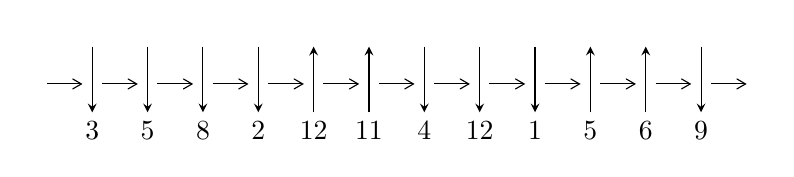
\begin{tikzpicture}[x=20pt, y=17pt]
	% nodes
	\node (C0) at (0, 0) {};
	\node (C1) at (1, 0) {};
	\node (C1U) at (1, +1) {};
	\node (C1D) at (1, -1) {3};

	\node (C2) at (2, 0) {};
	\node (C2U) at (2, +1) {};
	\node (C2D) at (2, -1) {5};

	\node (C3) at (3, 0) {};
	\node (C3U) at (3, +1) {};
	\node (C3D) at (3, -1) {8};

	\node (C4) at (4, 0) {};
	\node (C4U) at (4, +1) {};
	\node (C4D) at (4, -1) {2};

	\node (C5) at (5, 0) {};
	\node (C5U) at (5, +1) {};
	\node (C5D) at (5, -1) {12};

	\node (C6) at (6, 0) {};
	\node (C6U) at (6, +1) {};
	\node (C6D) at (6, -1) {11};

	\node (C7) at (7, 0) {};
	\node (C7U) at (7, +1) {};
	\node (C7D) at (7, -1) {4};

	\node (C8) at (8, 0) {};
	\node (C8U) at (8, +1) {};
	\node (C8D) at (8, -1) {12};

	\node (C9) at (9, 0) {};
	\node (C9U) at (9, +1) {};
	\node (C9D) at (9, -1) {1};

	\node (C10) at (10, 0) {};
	\node (C10U) at (10, +1) {};
	\node (C10D) at (10, -1) {5};

	\node (C11) at (11, 0) {};
	\node (C11U) at (11, +1) {};
	\node (C11D) at (11, -1) {6};

	\node (C12) at (12, 0) {};
	\node (C12U) at (12, +1) {};
	\node (C12D) at (12, -1) {9};
	\node (C13) at (13, 0) {};

	% arrows
	\draw[->,>={angle 60}]
	(C0) edge (C1) (C1) edge (C2) (C2) edge (C3) (C3) edge (C4) (C4) edge (C5) (C5) edge (C6) (C6) edge (C7) (C7) edge (C8) (C8) edge (C9) (C9) edge (C10) (C10) edge (C11) (C11) edge (C12) (C12) edge (C13) ;	\draw[->,>=stealth]
	(C1U) edge (C1D) (C2U) edge (C2D) (C3U) edge (C3D) (C4U) edge (C4D) (C5D) edge (C5U) (C6D) edge (C6U) (C7U) edge (C7D) (C8U) edge (C8D) (C9U) edge (C9D) (C10D) edge (C10U) (C11D) edge (C11U) (C12U) edge (C12D) ;
	\end{tikzpicture} \\
\hhline{~~} \\& 
\textbf{Solving Sequence} \\ \cline{2-2} 
 &
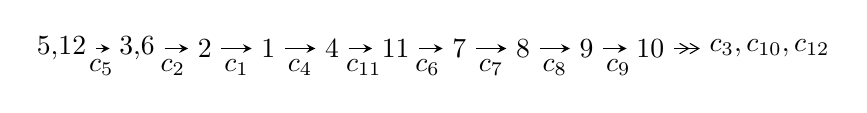
\begin{tikzpicture}[x=23pt, y=7pt]
	% node
	\node (A0) at (-1/8, 0) {5,12};
	\node (A1) at (17/16, 0) {3,6};
	\node (A2) at (17/8, 0) {2};
	\node (A3) at (25/8, 0) {1};
	\node (A4) at (33/8, 0) {4};
	\node (A5) at (41/8, 0) {11};
	\node (A6) at (49/8, 0) {7};
	\node (A7) at (57/8, 0) {8};
	\node (A8) at (65/8, 0) {9};
	\node (A9) at (73/8, 0) {10};
	\node (C1) at (1/2, -1) {$c_{5}$};
	\node (C2) at (13/8, -1) {$c_{2}$};
	\node (C3) at (21/8, -1) {$c_{1}$};
	\node (C4) at (29/8, -1) {$c_{4}$};
	\node (C5) at (37/8, -1) {$c_{11}$};
	\node (C6) at (45/8, -1) {$c_{6}$};
	\node (C7) at (53/8, -1) {$c_{7}$};
	\node (C8) at (61/8, -1) {$c_{8}$};
	\node (C9) at (69/8, -1) {$c_{9}$};
	\node (A10) at (11, 0) {$c_{3},c_{10},c_{12}$};

	% edge
	\draw[->,>=stealth]	
	(A0) edge (A1) (A1) edge (A2) (A2) edge (A3) (A3) edge (A4) (A4) edge (A5) (A5) edge (A6) (A6) edge (A7) (A7) edge (A8) (A8) edge (A9) ;
	\draw[->>,>={angle 60}]	
	(A9) edge (A10);
\end{tikzpicture} \\ 

\end{tabular} \\

\footnotetext{
The image of knot diagram is generated by the software ``\textbf{Draw programme}" developed by Andrew Bartholomew(\url{http://www.layer8.co.uk/maths/draw/index.htm\#Running-draw}), where we modified some parts for our purpose(\url{https://github.com/CATsTAILs/LinksPainter}).
}\phantom \\ \newline 
\centering \textbf{Ideals for irreducible components\footnotemark of $X_{\text{par}}$} 
 
\begin{align*}
I^u_{1}&=\langle 
5.91245\times10^{25} u^{28}+1.63252\times10^{26} u^{27}+\cdots+3.02573\times10^{27} b+2.88635\times10^{27},\\
\phantom{I^u_{1}}&\phantom{= \langle  }-5.15849\times10^{26} u^{28}-3.76417\times10^{26} u^{27}+\cdots+1.81544\times10^{28} a-1.59875\times10^{28},\\
\phantom{I^u_{1}}&\phantom{= \langle  }u^{29}+2 u^{28}+\cdots+24 u+8\rangle \\
I^u_{2}&=\langle 
-4 a^2 u-6 a^2+8 a u+17 b+12 a-2 u-20,\;4 a^3-6 a^2 u-8 a^2+2 a u+u-6,\;u^2+2\rangle \\
I^u_{3}&=\langle 
b+1,\;3 a-2 u-1,\;u^2+u+1\rangle \\
\\
I^v_{1}&=\langle 
a,\;- v^2+b-3 v+1,\;v^3+2 v^2-3 v+1\rangle \\
\end{align*}
\raggedright * 4 irreducible components of $\dim_{\mathbb{C}}=0$, with total 40 representations.\\
\footnotetext{All coefficients of polynomials are rational numbers. But the coefficients are sometimes approximated in decimal forms when there is not enough margin.}
\newpage
\renewcommand{\arraystretch}{1}
\centering \section*{I. $I^u_{1}= \langle 5.91\times10^{25} u^{28}+1.63\times10^{26} u^{27}+\cdots+3.03\times10^{27} b+2.89\times10^{27},\;-5.16\times10^{26} u^{28}-3.76\times10^{26} u^{27}+\cdots+1.82\times10^{28} a-1.60\times10^{28},\;u^{29}+2 u^{28}+\cdots+24 u+8 \rangle$}
\flushleft \textbf{(i) Arc colorings}\\
\begin{tabular}{m{7pt} m{180pt} m{7pt} m{180pt} }
\flushright $a_{5}=$&$\begin{pmatrix}1\\0\end{pmatrix}$ \\
\flushright $a_{12}=$&$\begin{pmatrix}0\\u\end{pmatrix}$ \\
\flushright $a_{3}=$&$\begin{pmatrix}0.0284146 u^{28}+0.0207342 u^{27}+\cdots-6.48402 u+0.880639\\-0.0195406 u^{28}-0.0539545 u^{27}+\cdots-0.120108 u-0.953934\end{pmatrix}$ \\
\flushright $a_{6}=$&$\begin{pmatrix}1\\- u^2\end{pmatrix}$ \\
\flushright $a_{2}=$&$\begin{pmatrix}0.00887400 u^{28}-0.0332203 u^{27}+\cdots-6.60412 u-0.0732946\\-0.0195406 u^{28}-0.0539545 u^{27}+\cdots-0.120108 u-0.953934\end{pmatrix}$ \\
\flushright $a_{1}=$&$\begin{pmatrix}-0.00109364 u^{28}+0.00268100 u^{27}+\cdots-2.31580 u-1.18662\\-0.0151700 u^{28}-0.0423430 u^{27}+\cdots+2.22414 u+0.186334\end{pmatrix}$ \\
\flushright $a_{4}=$&$\begin{pmatrix}0.0301055 u^{28}+0.0216495 u^{27}+\cdots-8.00531 u+0.779890\\-0.0370743 u^{28}-0.0881628 u^{27}+\cdots+0.425213 u-0.704192\end{pmatrix}$ \\
\flushright $a_{11}=$&$\begin{pmatrix}- u\\u^3+u\end{pmatrix}$ \\
\flushright $a_{7}=$&$\begin{pmatrix}u^2+1\\- u^4-2 u^2\end{pmatrix}$ \\
\flushright $a_{8}=$&$\begin{pmatrix}-0.0385391 u^{28}-0.0826420 u^{27}+\cdots+2.43382 u-0.756874\\0.0271306 u^{28}+0.0472982 u^{27}+\cdots-2.96732 u-0.287921\end{pmatrix}$ \\
\flushright $a_{9}=$&$\begin{pmatrix}-0.0385391 u^{28}-0.0826420 u^{27}+\cdots+2.43382 u-0.756874\\0.0222755 u^{28}+0.0429799 u^{27}+\cdots-2.52548 u-0.243412\end{pmatrix}$ \\
\flushright $a_{10}=$&$\begin{pmatrix}u^3+2 u\\- u^3- u\end{pmatrix}$\\&\end{tabular}
\flushleft \textbf{(ii) Obstruction class $= -1$}\\~\\
\flushleft \textbf{(iii) Cusp Shapes $= -\frac{5380338557971956323782944785}{27231580801980091699413843348} u^{28}-\frac{382789047733408314358823614}{756432800055002547205940093} u^{27}+\cdots-\frac{24975710409590861685346874876}{6807895200495022924853460837} u-\frac{79653205793763175879382867786}{6807895200495022924853460837}$}\\~\\
\newpage\renewcommand{\arraystretch}{1}
\flushleft \textbf{(iv) u-Polynomials at the component}\newline \\
\begin{tabular}{m{50pt}|m{274pt}}
Crossings & \hspace{64pt}u-Polynomials at each crossing \\
\hline $$\begin{aligned}c_{1}\end{aligned}$$&$\begin{aligned}
&u^{29}+24 u^{28}+\cdots-533 u+81
\end{aligned}$\\
\hline $$\begin{aligned}c_{2},c_{4}\end{aligned}$$&$\begin{aligned}
&u^{29}-6 u^{28}+\cdots+5 u-9
\end{aligned}$\\
\hline $$\begin{aligned}c_{3},c_{7}\end{aligned}$$&$\begin{aligned}
&u^{29}+2 u^{28}+\cdots+36 u-36
\end{aligned}$\\
\hline $$\begin{aligned}c_{5},c_{6},c_{11}\end{aligned}$$&$\begin{aligned}
&u^{29}+2 u^{28}+\cdots+24 u+8
\end{aligned}$\\
\hline $$\begin{aligned}c_{8},c_{9},c_{12}\end{aligned}$$&$\begin{aligned}
&u^{29}+5 u^{28}+\cdots+371 u-49
\end{aligned}$\\
\hline $$\begin{aligned}c_{10}\end{aligned}$$&$\begin{aligned}
&u^{29}-2 u^{28}+\cdots+109624 u+17960
\end{aligned}$\\
\hline
\end{tabular}\\~\\
\newpage\renewcommand{\arraystretch}{1}
\flushleft \textbf{(v) Riley Polynomials at the component}\newline \\
\begin{tabular}{m{50pt}|m{274pt}}
Crossings & \hspace{64pt}Riley Polynomials at each crossing \\
\hline $$\begin{aligned}c_{1}\end{aligned}$$&$\begin{aligned}
&y^{29}-32 y^{28}+\cdots+729751 y-6561
\end{aligned}$\\
\hline $$\begin{aligned}c_{2},c_{4}\end{aligned}$$&$\begin{aligned}
&y^{29}-24 y^{28}+\cdots-533 y-81
\end{aligned}$\\
\hline $$\begin{aligned}c_{3},c_{7}\end{aligned}$$&$\begin{aligned}
&y^{29}-6 y^{28}+\cdots+7416 y-1296
\end{aligned}$\\
\hline $$\begin{aligned}c_{5},c_{6},c_{11}\end{aligned}$$&$\begin{aligned}
&y^{29}+42 y^{28}+\cdots+1472 y-64
\end{aligned}$\\
\hline $$\begin{aligned}c_{8},c_{9},c_{12}\end{aligned}$$&$\begin{aligned}
&y^{29}-39 y^{28}+\cdots+313551 y-2401
\end{aligned}$\\
\hline $$\begin{aligned}c_{10}\end{aligned}$$&$\begin{aligned}
&y^{29}+126 y^{28}+\cdots+874175296 y-322561600
\end{aligned}$\\
\hline
\end{tabular}\\~\\
\newpage\flushleft \textbf{(vi) Complex Volumes and Cusp Shapes}
$$\begin{array}{c|c|c}  
\text{Solutions to }I^u_{1}& \I (\text{vol} + \sqrt{-1}CS) & \text{Cusp shape}\\
 \hline 
\begin{aligned}
u &= \phantom{-}0.056486 + 1.108600 I \\
a &= \phantom{-}0.509763 + 0.504736 I \\
b &= \phantom{-}0.907095 - 0.525537 I\end{aligned}
 & -1.48252 + 4.21157 I & -5.04918 - 7.08997 I \\ \hline\begin{aligned}
u &= \phantom{-}0.056486 - 1.108600 I \\
a &= \phantom{-}0.509763 - 0.504736 I \\
b &= \phantom{-}0.907095 + 0.525537 I\end{aligned}
 & -1.48252 - 4.21157 I & -5.04918 + 7.08997 I \\ \hline\begin{aligned}
u &= -0.388139 + 1.131690 I \\
a &= \phantom{-}0.13323 + 1.59492 I \\
b &= -0.279564 - 0.842912 I\end{aligned}
 & -6.31420 - 2.62388 I & -7.82173 + 3.53782 I \\ \hline\begin{aligned}
u &= -0.388139 - 1.131690 I \\
a &= \phantom{-}0.13323 - 1.59492 I \\
b &= -0.279564 + 0.842912 I\end{aligned}
 & -6.31420 + 2.62388 I & -7.82173 - 3.53782 I \\ \hline\begin{aligned}
u &= -1.26121\phantom{ +0.000000I} \\
a &= -1.32815\phantom{ +0.000000I} \\
b &= \phantom{-}1.48540\phantom{ +0.000000I}\end{aligned}
 & -8.96674\phantom{ +0.000000I} & -10.0380\phantom{ +0.000000I} \\ \hline\begin{aligned}
u &= \phantom{-}0.596916 + 1.218910 I \\
a &= -0.248187 + 0.135692 I \\
b &= \phantom{-}1.167880 + 0.296850 I\end{aligned}
 & -1.89970 + 1.08021 I & -8.90087 + 2.30906 I \\ \hline\begin{aligned}
u &= \phantom{-}0.596916 - 1.218910 I \\
a &= -0.248187 - 0.135692 I \\
b &= \phantom{-}1.167880 - 0.296850 I\end{aligned}
 & -1.89970 - 1.08021 I & -8.90087 - 2.30906 I \\ \hline\begin{aligned}
u &= \phantom{-}0.246173 + 0.558581 I \\
a &= \phantom{-}0.428232 - 0.225932 I \\
b &= \phantom{-}0.080951 + 0.316217 I\end{aligned}
 & -0.137288 + 1.167630 I & -1.98849 - 5.87802 I \\ \hline\begin{aligned}
u &= \phantom{-}0.246173 - 0.558581 I \\
a &= \phantom{-}0.428232 + 0.225932 I \\
b &= \phantom{-}0.080951 - 0.316217 I\end{aligned}
 & -0.137288 - 1.167630 I & -1.98849 + 5.87802 I \\ \hline\begin{aligned}
u &= \phantom{-}0.229637 + 1.393650 I \\
a &= -0.24130 - 1.45930 I \\
b &= -1.306470 + 0.114811 I\end{aligned}
 & -9.08630 + 0.60306 I & -9.48302 + 0.55490 I\\
 \hline 
 \end{array}$$\newpage$$\begin{array}{c|c|c}  
\text{Solutions to }I^u_{1}& \I (\text{vol} + \sqrt{-1}CS) & \text{Cusp shape}\\
 \hline 
\begin{aligned}
u &= \phantom{-}0.229637 - 1.393650 I \\
a &= -0.24130 + 1.45930 I \\
b &= -1.306470 - 0.114811 I\end{aligned}
 & -9.08630 - 0.60306 I & -9.48302 - 0.55490 I \\ \hline\begin{aligned}
u &= -0.92622 + 1.09424 I \\
a &= -0.679131 - 1.154340 I \\
b &= \phantom{-}1.50364 + 0.34882 I\end{aligned}
 & -12.14260 - 7.09236 I & -9.88548 + 4.43112 I \\ \hline\begin{aligned}
u &= -0.92622 - 1.09424 I \\
a &= -0.679131 + 1.154340 I \\
b &= \phantom{-}1.50364 - 0.34882 I\end{aligned}
 & -12.14260 + 7.09236 I & -9.88548 - 4.43112 I \\ \hline\begin{aligned}
u &= \phantom{-}0.032332 + 0.523301 I \\
a &= -2.28494 + 0.79922 I \\
b &= -1.045540 - 0.191235 I\end{aligned}
 & -2.84144 - 0.79516 I & -13.03610 - 2.36785 I \\ \hline\begin{aligned}
u &= \phantom{-}0.032332 - 0.523301 I \\
a &= -2.28494 - 0.79922 I \\
b &= -1.045540 + 0.191235 I\end{aligned}
 & -2.84144 + 0.79516 I & -13.03610 + 2.36785 I \\ \hline\begin{aligned}
u &= -0.06536 + 1.54556 I \\
a &= \phantom{-}0.658215 - 0.546986 I \\
b &= -0.451198 + 0.592359 I\end{aligned}
 & -7.37261 + 1.38935 I & -7.45295 - 4.42658 I \\ \hline\begin{aligned}
u &= -0.06536 - 1.54556 I \\
a &= \phantom{-}0.658215 + 0.546986 I \\
b &= -0.451198 - 0.592359 I\end{aligned}
 & -7.37261 - 1.38935 I & -7.45295 + 4.42658 I \\ \hline\begin{aligned}
u &= \phantom{-}0.434195 + 0.049760 I \\
a &= -0.72855 - 1.30157 I \\
b &= \phantom{-}0.901341 + 0.657097 I\end{aligned}
 & \phantom{-}1.84827 - 2.56654 I & \phantom{-}3.67854 + 0.07862 I \\ \hline\begin{aligned}
u &= \phantom{-}0.434195 - 0.049760 I \\
a &= -0.72855 + 1.30157 I \\
b &= \phantom{-}0.901341 - 0.657097 I\end{aligned}
 & \phantom{-}1.84827 + 2.56654 I & \phantom{-}3.67854 - 0.07862 I \\ \hline\begin{aligned}
u &= -0.352396\phantom{ +0.000000I} \\
a &= \phantom{-}5.25680\phantom{ +0.000000I} \\
b &= -0.489012\phantom{ +0.000000I}\end{aligned}
 & -2.50392\phantom{ +0.000000I} & \phantom{-}5.38240\phantom{ +0.000000I}\\
 \hline 
 \end{array}$$\newpage$$\begin{array}{c|c|c}  
\text{Solutions to }I^u_{1}& \I (\text{vol} + \sqrt{-1}CS) & \text{Cusp shape}\\
 \hline 
\begin{aligned}
u &= -0.210444\phantom{ +0.000000I} \\
a &= \phantom{-}3.27498\phantom{ +0.000000I} \\
b &= -0.852919\phantom{ +0.000000I}\end{aligned}
 & -1.24667\phantom{ +0.000000I} & -7.81580\phantom{ +0.000000I} \\ \hline\begin{aligned}
u &= -0.31071 + 1.78442 I \\
a &= -0.039698 - 1.223290 I \\
b &= \phantom{-}1.49818 + 0.64361 I\end{aligned}
 & \phantom{-}17.7563 - 12.2354 I & \phantom{-0.000000 } 0 \\ \hline\begin{aligned}
u &= -0.31071 - 1.78442 I \\
a &= -0.039698 + 1.223290 I \\
b &= \phantom{-}1.49818 - 0.64361 I\end{aligned}
 & \phantom{-}17.7563 + 12.2354 I & \phantom{-0.000000 } 0 \\ \hline\begin{aligned}
u &= -0.14116 + 1.80910 I \\
a &= -0.144818 + 1.112790 I \\
b &= -0.015590 - 1.360440 I\end{aligned}
 & -16.9778 - 5.1847 I & \phantom{-0.000000 } 0 \\ \hline\begin{aligned}
u &= -0.14116 - 1.80910 I \\
a &= -0.144818 - 1.112790 I \\
b &= -0.015590 + 1.360440 I\end{aligned}
 & -16.9778 + 5.1847 I & \phantom{-0.000000 } 0 \\ \hline\begin{aligned}
u &= \phantom{-}0.04856 + 1.88123 I \\
a &= \phantom{-}0.226652 - 0.888720 I \\
b &= -1.55643 + 0.68836 I\end{aligned}
 & \phantom{-}17.7608 + 2.1451 I & \phantom{-0.000000 } 0 \\ \hline\begin{aligned}
u &= \phantom{-}0.04856 - 1.88123 I \\
a &= \phantom{-}0.226652 + 0.888720 I \\
b &= -1.55643 - 0.68836 I\end{aligned}
 & \phantom{-}17.7608 - 2.1451 I & \phantom{-0.000000 } 0 \\ \hline\begin{aligned}
u &= \phantom{-}0.09931 + 1.89084 I \\
a &= -0.024622 + 0.392844 I \\
b &= \phantom{-}1.52399 - 0.23863 I\end{aligned}
 & -13.8756 + 4.6395 I & \phantom{-0.000000 } 0 \\ \hline\begin{aligned}
u &= \phantom{-}0.09931 - 1.89084 I \\
a &= -0.024622 - 0.392844 I \\
b &= \phantom{-}1.52399 + 0.23863 I\end{aligned}
 & -13.8756 - 4.6395 I & \phantom{-0.000000 } 0\\
 \hline 
 \end{array}$$\newpage\newpage\renewcommand{\arraystretch}{1}
\centering \section*{II. $I^u_{2}= \langle -4 a^2 u-6 a^2+8 a u+17 b+12 a-2 u-20,\;4 a^3-6 a^2 u-8 a^2+2 a u+u-6,\;u^2+2 \rangle$}
\flushleft \textbf{(i) Arc colorings}\\
\begin{tabular}{m{7pt} m{180pt} m{7pt} m{180pt} }
\flushright $a_{5}=$&$\begin{pmatrix}1\\0\end{pmatrix}$ \\
\flushright $a_{12}=$&$\begin{pmatrix}0\\u\end{pmatrix}$ \\
\flushright $a_{3}=$&$\begin{pmatrix}a\\0.235294 a^{2} u-0.470588 a u+\cdots-0.705882 a+1.17647\end{pmatrix}$ \\
\flushright $a_{6}=$&$\begin{pmatrix}1\\2\end{pmatrix}$ \\
\flushright $a_{2}=$&$\begin{pmatrix}0.235294 a^{2} u-0.470588 a u+\cdots+0.294118 a+1.17647\\0.235294 a^{2} u-0.470588 a u+\cdots-0.705882 a+1.17647\end{pmatrix}$ \\
\flushright $a_{1}=$&$\begin{pmatrix}\frac{1}{2} u\\0.352941 a^{2} u+0.294118 a u+\cdots+0.941176 a+1.76471\end{pmatrix}$ \\
\flushright $a_{4}=$&$\begin{pmatrix}-0.411765 a^{2} u+0.823529 a u+\cdots+0.235294 a-0.0588235\\0.117647 a^{2} u+0.764706 a u+\cdots+1.64706 a-0.411765\end{pmatrix}$ \\
\flushright $a_{11}=$&$\begin{pmatrix}- u\\- u\end{pmatrix}$ \\
\flushright $a_{7}=$&$\begin{pmatrix}-1\\0\end{pmatrix}$ \\
\flushright $a_{8}=$&$\begin{pmatrix}\frac{1}{2} u\\0.352941 a^{2} u+0.294118 a u+\cdots+0.941176 a+1.76471\end{pmatrix}$ \\
\flushright $a_{9}=$&$\begin{pmatrix}\frac{1}{2} u\\0.352941 a^{2} u+0.294118 a u+\cdots+0.941176 a+1.76471\end{pmatrix}$ \\
\flushright $a_{10}=$&$\begin{pmatrix}0\\- u\end{pmatrix}$\\&\end{tabular}
\flushleft \textbf{(ii) Obstruction class $= 1$}\\~\\
\flushleft \textbf{(iii) Cusp Shapes $= \frac{16}{17} a^2 u+\frac{24}{17} a^2-\frac{32}{17} a u-\frac{48}{17} a+\frac{8}{17} u-\frac{124}{17}$}\\~\\
\newpage\renewcommand{\arraystretch}{1}
\flushleft \textbf{(iv) u-Polynomials at the component}\newline \\
\begin{tabular}{m{50pt}|m{274pt}}
Crossings & \hspace{64pt}u-Polynomials at each crossing \\
\hline $$\begin{aligned}c_{1},c_{7}\end{aligned}$$&$\begin{aligned}
&(u^3- u^2+2 u-1)^2
\end{aligned}$\\
\hline $$\begin{aligned}c_{2}\end{aligned}$$&$\begin{aligned}
&(u^3+u^2-1)^2
\end{aligned}$\\
\hline $$\begin{aligned}c_{3}\end{aligned}$$&$\begin{aligned}
&(u^3+u^2+2 u+1)^2
\end{aligned}$\\
\hline $$\begin{aligned}c_{4}\end{aligned}$$&$\begin{aligned}
&(u^3- u^2+1)^2
\end{aligned}$\\
\hline $$\begin{aligned}c_{5},c_{6},c_{10}\\c_{11}\end{aligned}$$&$\begin{aligned}
&(u^2+2)^3
\end{aligned}$\\
\hline $$\begin{aligned}c_{8},c_{9}\end{aligned}$$&$\begin{aligned}
&(u+1)^6
\end{aligned}$\\
\hline $$\begin{aligned}c_{12}\end{aligned}$$&$\begin{aligned}
&(u-1)^6
\end{aligned}$\\
\hline
\end{tabular}\\~\\
\newpage\renewcommand{\arraystretch}{1}
\flushleft \textbf{(v) Riley Polynomials at the component}\newline \\
\begin{tabular}{m{50pt}|m{274pt}}
Crossings & \hspace{64pt}Riley Polynomials at each crossing \\
\hline $$\begin{aligned}c_{1},c_{3},c_{7}\end{aligned}$$&$\begin{aligned}
&(y^3+3 y^2+2 y-1)^2
\end{aligned}$\\
\hline $$\begin{aligned}c_{2},c_{4}\end{aligned}$$&$\begin{aligned}
&(y^3- y^2+2 y-1)^2
\end{aligned}$\\
\hline $$\begin{aligned}c_{5},c_{6},c_{10}\\c_{11}\end{aligned}$$&$\begin{aligned}
&(y+2)^6
\end{aligned}$\\
\hline $$\begin{aligned}c_{8},c_{9},c_{12}\end{aligned}$$&$\begin{aligned}
&(y-1)^6
\end{aligned}$\\
\hline
\end{tabular}\\~\\
\newpage\flushleft \textbf{(vi) Complex Volumes and Cusp Shapes}
$$\begin{array}{c|c|c}  
\text{Solutions to }I^u_{2}& \I (\text{vol} + \sqrt{-1}CS) & \text{Cusp shape}\\
 \hline 
\begin{aligned}
u &= \phantom{-0.000000 -}1.414210 I \\
a &= \phantom{-}0.520153 + 0.983610 I \\
b &= \phantom{-}0.877439 - 0.744862 I\end{aligned}
 & -3.55561 + 2.82812 I & -8.49024 - 2.97945 I \\ \hline\begin{aligned}
u &= \phantom{-0.000000 -}1.414210 I \\
a &= -0.275030 - 0.506114 I \\
b &= \phantom{-}0.877439 + 0.744862 I\end{aligned}
 & -3.55561 - 2.82812 I & -8.49024 + 2.97945 I \\ \hline\begin{aligned}
u &= \phantom{-0.000000 -}1.414210 I \\
a &= \phantom{-}1.75488 + 1.64382 I \\
b &= -0.754878\phantom{ +0.000000I}\end{aligned}
 & -7.69319\phantom{ +0.000000I} & -15.0195 + 0. I\phantom{ +0.000000I} \\ \hline\begin{aligned}
u &= \phantom{-0.000000 } -1.414210 I \\
a &= \phantom{-}0.520153 - 0.983610 I \\
b &= \phantom{-}0.877439 + 0.744862 I\end{aligned}
 & -3.55561 - 2.82812 I & -8.49024 + 2.97945 I \\ \hline\begin{aligned}
u &= \phantom{-0.000000 } -1.414210 I \\
a &= -0.275030 + 0.506114 I \\
b &= \phantom{-}0.877439 - 0.744862 I\end{aligned}
 & -3.55561 + 2.82812 I & -8.49024 - 2.97945 I \\ \hline\begin{aligned}
u &= \phantom{-0.000000 } -1.414210 I \\
a &= \phantom{-}1.75488 - 1.64382 I \\
b &= -0.754878\phantom{ +0.000000I}\end{aligned}
 & -7.69319\phantom{ +0.000000I} & -15.0195 + 0. I\phantom{ +0.000000I}\\
 \hline 
 \end{array}$$\newpage\newpage\renewcommand{\arraystretch}{1}
\centering \section*{III. $I^u_{3}= \langle b+1,\;3 a-2 u-1,\;u^2+u+1 \rangle$}
\flushleft \textbf{(i) Arc colorings}\\
\begin{tabular}{m{7pt} m{180pt} m{7pt} m{180pt} }
\flushright $a_{5}=$&$\begin{pmatrix}1\\0\end{pmatrix}$ \\
\flushright $a_{12}=$&$\begin{pmatrix}0\\u\end{pmatrix}$ \\
\flushright $a_{3}=$&$\begin{pmatrix}\frac{2}{3} u+\frac{1}{3}\\-1\end{pmatrix}$ \\
\flushright $a_{6}=$&$\begin{pmatrix}1\\u+1\end{pmatrix}$ \\
\flushright $a_{2}=$&$\begin{pmatrix}\frac{2}{3} u-\frac{2}{3}\\-1\end{pmatrix}$ \\
\flushright $a_{1}=$&$\begin{pmatrix}-1\\0\end{pmatrix}$ \\
\flushright $a_{4}=$&$\begin{pmatrix}\frac{2}{3} u+\frac{1}{3}\\-1\end{pmatrix}$ \\
\flushright $a_{11}=$&$\begin{pmatrix}- u\\u+1\end{pmatrix}$ \\
\flushright $a_{7}=$&$\begin{pmatrix}- u\\u+2\end{pmatrix}$ \\
\flushright $a_{8}=$&$\begin{pmatrix}- u\\u+2\end{pmatrix}$ \\
\flushright $a_{9}=$&$\begin{pmatrix}- u\\u+1\end{pmatrix}$ \\
\flushright $a_{10}=$&$\begin{pmatrix}-2 u-1\\u+1\end{pmatrix}$\\&\end{tabular}
\flushleft \textbf{(ii) Obstruction class $= 1$}\\~\\
\flushleft \textbf{(iii) Cusp Shapes $= \frac{20}{3} u-3$}\\~\\
\newpage\renewcommand{\arraystretch}{1}
\flushleft \textbf{(iv) u-Polynomials at the component}\newline \\
\begin{tabular}{m{50pt}|m{274pt}}
Crossings & \hspace{64pt}u-Polynomials at each crossing \\
\hline $$\begin{aligned}c_{1},c_{2}\end{aligned}$$&$\begin{aligned}
&(u-1)^2
\end{aligned}$\\
\hline $$\begin{aligned}c_{3},c_{7}\end{aligned}$$&$\begin{aligned}
&u^2
\end{aligned}$\\
\hline $$\begin{aligned}c_{4}\end{aligned}$$&$\begin{aligned}
&(u+1)^2
\end{aligned}$\\
\hline $$\begin{aligned}c_{5},c_{6},c_{10}\\c_{12}\end{aligned}$$&$\begin{aligned}
&u^2+u+1
\end{aligned}$\\
\hline $$\begin{aligned}c_{8},c_{9},c_{11}\end{aligned}$$&$\begin{aligned}
&u^2- u+1
\end{aligned}$\\
\hline
\end{tabular}\\~\\
\newpage\renewcommand{\arraystretch}{1}
\flushleft \textbf{(v) Riley Polynomials at the component}\newline \\
\begin{tabular}{m{50pt}|m{274pt}}
Crossings & \hspace{64pt}Riley Polynomials at each crossing \\
\hline $$\begin{aligned}c_{1},c_{2},c_{4}\end{aligned}$$&$\begin{aligned}
&(y-1)^2
\end{aligned}$\\
\hline $$\begin{aligned}c_{3},c_{7}\end{aligned}$$&$\begin{aligned}
&y^2
\end{aligned}$\\
\hline $$\begin{aligned}c_{5},c_{6},c_{8}\\c_{9},c_{10},c_{11}\\c_{12}\end{aligned}$$&$\begin{aligned}
&y^2+y+1
\end{aligned}$\\
\hline
\end{tabular}\\~\\
\newpage\flushleft \textbf{(vi) Complex Volumes and Cusp Shapes}
$$\begin{array}{c|c|c}  
\text{Solutions to }I^u_{3}& \I (\text{vol} + \sqrt{-1}CS) & \text{Cusp shape}\\
 \hline 
\begin{aligned}
u &= -0.500000 + 0.866025 I \\
a &= \phantom{-0.000000 -}0.577350 I \\
b &= -1.00000\phantom{ +0.000000I}\end{aligned}
 & -1.64493 - 2.02988 I & -6.33333 + 5.77350 I \\ \hline\begin{aligned}
u &= -0.500000 - 0.866025 I \\
a &= \phantom{-0.000000 } -0.577350 I \\
b &= -1.00000\phantom{ +0.000000I}\end{aligned}
 & -1.64493 + 2.02988 I & -6.33333 - 5.77350 I\\
 \hline 
 \end{array}$$\newpage\newpage\renewcommand{\arraystretch}{1}
\centering \section*{IV. $I^v_{1}= \langle a,\;- v^2+b-3 v+1,\;v^3+2 v^2-3 v+1 \rangle$}
\flushleft \textbf{(i) Arc colorings}\\
\begin{tabular}{m{7pt} m{180pt} m{7pt} m{180pt} }
\flushright $a_{5}=$&$\begin{pmatrix}1\\0\end{pmatrix}$ \\
\flushright $a_{12}=$&$\begin{pmatrix}v\\0\end{pmatrix}$ \\
\flushright $a_{3}=$&$\begin{pmatrix}0\\v^2+3 v-1\end{pmatrix}$ \\
\flushright $a_{6}=$&$\begin{pmatrix}1\\0\end{pmatrix}$ \\
\flushright $a_{2}=$&$\begin{pmatrix}v^2+3 v-1\\v^2+3 v-1\end{pmatrix}$ \\
\flushright $a_{1}=$&$\begin{pmatrix}v^2+3 v-1\\- v^2-2 v+3\end{pmatrix}$ \\
\flushright $a_{4}=$&$\begin{pmatrix}-2 v^2-5 v+4\\-2 v^2-5 v+3\end{pmatrix}$ \\
\flushright $a_{11}=$&$\begin{pmatrix}v\\0\end{pmatrix}$ \\
\flushright $a_{7}=$&$\begin{pmatrix}1\\0\end{pmatrix}$ \\
\flushright $a_{8}=$&$\begin{pmatrix}- v^2-3 v+1\\v^2+2 v-3\end{pmatrix}$ \\
\flushright $a_{9}=$&$\begin{pmatrix}- v^2-2 v+1\\v^2+2 v-3\end{pmatrix}$ \\
\flushright $a_{10}=$&$\begin{pmatrix}v\\0\end{pmatrix}$\\&\end{tabular}
\flushleft \textbf{(ii) Obstruction class $= 1$}\\~\\
\flushleft \textbf{(iii) Cusp Shapes $= 8 v^2+26 v-26$}\\~\\
\newpage\renewcommand{\arraystretch}{1}
\flushleft \textbf{(iv) u-Polynomials at the component}\newline \\
\begin{tabular}{m{50pt}|m{274pt}}
Crossings & \hspace{64pt}u-Polynomials at each crossing \\
\hline $$\begin{aligned}c_{1},c_{3}\end{aligned}$$&$\begin{aligned}
&u^3- u^2+2 u-1
\end{aligned}$\\
\hline $$\begin{aligned}c_{2}\end{aligned}$$&$\begin{aligned}
&u^3+u^2-1
\end{aligned}$\\
\hline $$\begin{aligned}c_{4}\end{aligned}$$&$\begin{aligned}
&u^3- u^2+1
\end{aligned}$\\
\hline $$\begin{aligned}c_{5},c_{6},c_{10}\\c_{11}\end{aligned}$$&$\begin{aligned}
&u^3
\end{aligned}$\\
\hline $$\begin{aligned}c_{7}\end{aligned}$$&$\begin{aligned}
&u^3+u^2+2 u+1
\end{aligned}$\\
\hline $$\begin{aligned}c_{8},c_{9}\end{aligned}$$&$\begin{aligned}
&(u-1)^3
\end{aligned}$\\
\hline $$\begin{aligned}c_{12}\end{aligned}$$&$\begin{aligned}
&(u+1)^3
\end{aligned}$\\
\hline
\end{tabular}\\~\\
\newpage\renewcommand{\arraystretch}{1}
\flushleft \textbf{(v) Riley Polynomials at the component}\newline \\
\begin{tabular}{m{50pt}|m{274pt}}
Crossings & \hspace{64pt}Riley Polynomials at each crossing \\
\hline $$\begin{aligned}c_{1},c_{3},c_{7}\end{aligned}$$&$\begin{aligned}
&y^3+3 y^2+2 y-1
\end{aligned}$\\
\hline $$\begin{aligned}c_{2},c_{4}\end{aligned}$$&$\begin{aligned}
&y^3- y^2+2 y-1
\end{aligned}$\\
\hline $$\begin{aligned}c_{5},c_{6},c_{10}\\c_{11}\end{aligned}$$&$\begin{aligned}
&y^3
\end{aligned}$\\
\hline $$\begin{aligned}c_{8},c_{9},c_{12}\end{aligned}$$&$\begin{aligned}
&(y-1)^3
\end{aligned}$\\
\hline
\end{tabular}\\~\\
\newpage\flushleft \textbf{(vi) Complex Volumes and Cusp Shapes}
$$\begin{array}{c|c|c}  
\text{Solutions to }I^v_{1}& \I (\text{vol} + \sqrt{-1}CS) & \text{Cusp shape}\\
 \hline 
\begin{aligned}
v &= \phantom{-}0.539798 + 0.182582 I \\
a &= \phantom{-0.000000 } 0 \\
b &= \phantom{-}0.877439 + 0.744862 I\end{aligned}
 & \phantom{-}1.37919 - 2.82812 I & -9.90089 + 6.32406 I \\ \hline\begin{aligned}
v &= \phantom{-}0.539798 - 0.182582 I \\
a &= \phantom{-0.000000 } 0 \\
b &= \phantom{-}0.877439 - 0.744862 I\end{aligned}
 & \phantom{-}1.37919 + 2.82812 I & -9.90089 - 6.32406 I \\ \hline\begin{aligned}
v &= -3.07960\phantom{ +0.000000I} \\
a &= \phantom{-0.000000 } 0 \\
b &= -0.754878\phantom{ +0.000000I}\end{aligned}
 & -2.75839\phantom{ +0.000000I} & -30.1980\phantom{ +0.000000I}\\
 \hline 
 \end{array}$$\newpage
\newpage\renewcommand{\arraystretch}{1}
\centering \section*{ V. u-Polynomials}
\begin{tabular}{m{50pt}|m{274pt}}
Crossings & \hspace{64pt}u-Polynomials at each crossing \\
\hline $$\begin{aligned}c_{1}\end{aligned}$$&$\begin{aligned}
&((u-1)^2)(u^3- u^2+2 u-1)^3(u^{29}+24 u^{28}+\cdots-533 u+81)
\end{aligned}$\\
\hline $$\begin{aligned}c_{2}\end{aligned}$$&$\begin{aligned}
&((u-1)^2)(u^3+u^2-1)^3(u^{29}-6 u^{28}+\cdots+5 u-9)
\end{aligned}$\\
\hline $$\begin{aligned}c_{3}\end{aligned}$$&$\begin{aligned}
&u^2(u^3- u^2+2 u-1)(u^3+u^2+2 u+1)^{2}(u^{29}+2 u^{28}+\cdots+36 u-36)
\end{aligned}$\\
\hline $$\begin{aligned}c_{4}\end{aligned}$$&$\begin{aligned}
&((u+1)^2)(u^3- u^2+1)^3(u^{29}-6 u^{28}+\cdots+5 u-9)
\end{aligned}$\\
\hline $$\begin{aligned}c_{5},c_{6}\end{aligned}$$&$\begin{aligned}
&u^3(u^2+2)^3(u^2+u+1)(u^{29}+2 u^{28}+\cdots+24 u+8)
\end{aligned}$\\
\hline $$\begin{aligned}c_{7}\end{aligned}$$&$\begin{aligned}
&u^2(u^3- u^2+2 u-1)^{2}(u^3+u^2+2 u+1)(u^{29}+2 u^{28}+\cdots+36 u-36)
\end{aligned}$\\
\hline $$\begin{aligned}c_{8},c_{9}\end{aligned}$$&$\begin{aligned}
&((u-1)^3)(u+1)^6(u^2- u+1)(u^{29}+5 u^{28}+\cdots+371 u-49)
\end{aligned}$\\
\hline $$\begin{aligned}c_{10}\end{aligned}$$&$\begin{aligned}
&u^3(u^2+2)^3(u^2+u+1)(u^{29}-2 u^{28}+\cdots+109624 u+17960)
\end{aligned}$\\
\hline $$\begin{aligned}c_{11}\end{aligned}$$&$\begin{aligned}
&u^3(u^2+2)^3(u^2- u+1)(u^{29}+2 u^{28}+\cdots+24 u+8)
\end{aligned}$\\
\hline $$\begin{aligned}c_{12}\end{aligned}$$&$\begin{aligned}
&((u-1)^6)(u+1)^3(u^2+u+1)(u^{29}+5 u^{28}+\cdots+371 u-49)
\end{aligned}$\\
\hline
\end{tabular}\newpage\renewcommand{\arraystretch}{1}
\centering \section*{ VI. Riley Polynomials}
\begin{tabular}{m{50pt}|m{274pt}}
Crossings & \hspace{64pt}Riley Polynomials at each crossing \\
\hline $$\begin{aligned}c_{1}\end{aligned}$$&$\begin{aligned}
&((y-1)^2)(y^3+3 y^2+2 y-1)^3(y^{29}-32 y^{28}+\cdots+729751 y-6561)
\end{aligned}$\\
\hline $$\begin{aligned}c_{2},c_{4}\end{aligned}$$&$\begin{aligned}
&((y-1)^2)(y^3- y^2+2 y-1)^3(y^{29}-24 y^{28}+\cdots-533 y-81)
\end{aligned}$\\
\hline $$\begin{aligned}c_{3},c_{7}\end{aligned}$$&$\begin{aligned}
&y^2(y^3+3 y^2+2 y-1)^3(y^{29}-6 y^{28}+\cdots+7416 y-1296)
\end{aligned}$\\
\hline $$\begin{aligned}c_{5},c_{6},c_{11}\end{aligned}$$&$\begin{aligned}
&y^3(y+2)^6(y^2+y+1)(y^{29}+42 y^{28}+\cdots+1472 y-64)
\end{aligned}$\\
\hline $$\begin{aligned}c_{8},c_{9},c_{12}\end{aligned}$$&$\begin{aligned}
&((y-1)^9)(y^2+y+1)(y^{29}-39 y^{28}+\cdots+313551 y-2401)
\end{aligned}$\\
\hline $$\begin{aligned}c_{10}\end{aligned}$$&$\begin{aligned}
&y^3(y+2)^6(y^2+y+1)\\
&\cdot(y^{29}+126 y^{28}+\cdots+874175296 y-322561600)
\end{aligned}$\\
\hline
\end{tabular}
\vskip 2pc
\end{document}